\documentclass[tikz,border=6pt]{standalone}

\usetikzlibrary{arrows.meta,fit,positioning}

\begin{document}
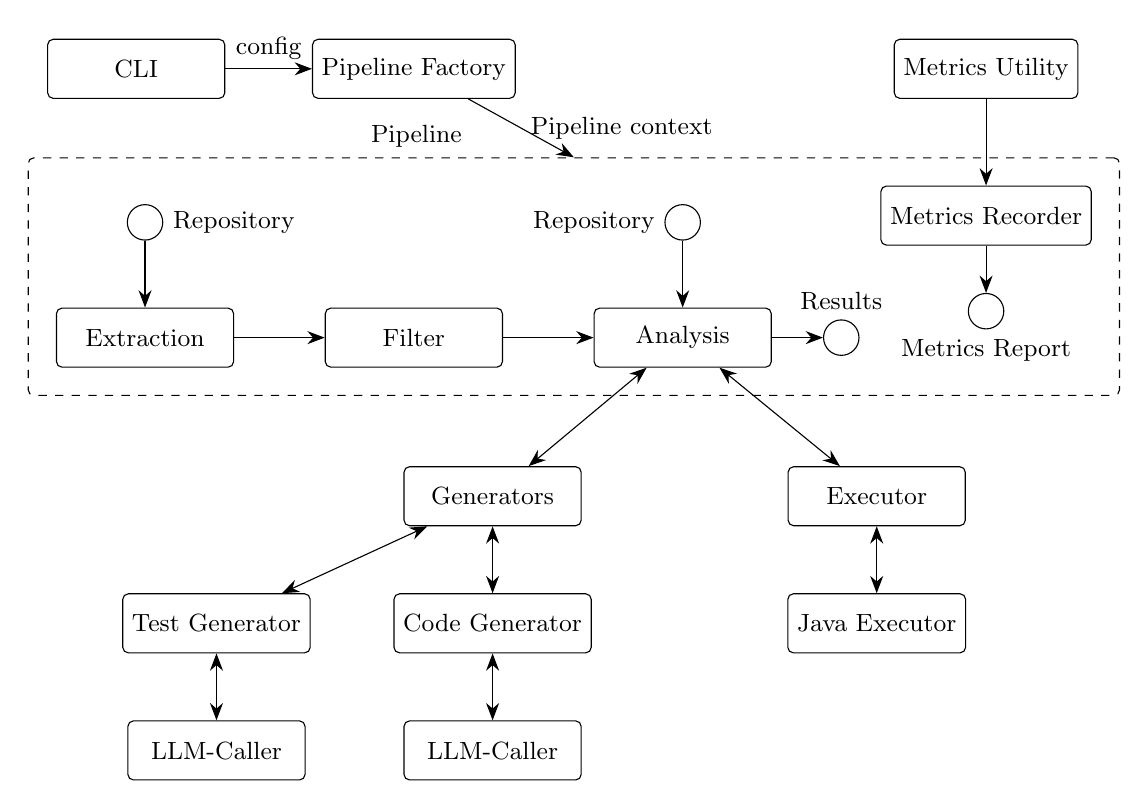
\begin{tikzpicture}[
    node distance=1.05cm and 1.25cm,
    box/.style={
        draw,
        rounded corners=2pt,
        minimum width=2.25cm,
        minimum height=0.75cm,
        align=center
    },
    put/.style={circle,draw,minimum size=0.45cm,inner sep=0pt},
    flow/.style={-{Stealth[length=2.2mm]}},
    interaction/.style={{Stealth[length=2.2mm]}-{Stealth[length=2.2mm]}},
    every node/.style={font=\small}
]
    \node[box] (cli) {CLI};
    \node[box, right=1.10cm of cli] (pipeline-factory) {Pipeline Factory};
    \node[box, right=4.80cm of pipeline-factory] (metrics-utility) {Metrics Utility};

    \node[box, below=2.65cm of pipeline-factory] (filter) {Filter};
    \node[box, left=1.15cm of filter] (extraction) {Extraction};
    \node[box, right=1.15cm of filter] (analysis) {Analysis};
    \node[put, above=0.85cm of extraction, label=right:Repository] (repo-extraction) {};
    \node[put, above=0.85cm of analysis, label=left:Repository] (repo-analysis) {};
    \node[put, right=0.65cm of analysis, label=above:Results] (results) {};

    \node[box, below=1.10cm of metrics-utility] (metrics-recorder) {Metrics Recorder};
    \node[put, below=0.60cm of metrics-recorder, label=below:Metrics Report] (metrics-report) {};

    \node[draw,dashed,rounded corners=2pt,
        fit=(repo-extraction)(repo-analysis)(extraction)(filter)(analysis)(results)
            (metrics-recorder)(metrics-report),
        inner sep=10pt,
        label={[xshift=-2.0cm]above:Pipeline}
    ] (pipeline-group) {};

    \node[box, below left=1.25cm and 0.15cm of analysis] (generators) {Generators};
    \node[box, below=0.85cm of generators] (code-generator) {Code Generator};
    \node[box, left=1.05cm of code-generator] (test-generator) {Test Generator};
    \node[box, below=0.85cm of test-generator] (llm-test) {LLM-Caller};
    \node[box, below=0.85cm of code-generator] (llm-code) {LLM-Caller};

    \node[box, below right=1.25cm and 0.20cm of analysis] (executor) {Executor};
    \node[box, below=0.85cm of executor] (java-executor) {Java Executor};

    \draw[flow] (cli) -- node[above] {config} (pipeline-factory);
    \draw[flow] (pipeline-factory) -- node[right] {Pipeline context} (pipeline-group.north);
    \draw[flow] (repo-extraction) -- (extraction);
    \draw[flow] (repo-analysis) -- (analysis);
    \draw[flow] (extraction) -- (filter);
    \draw[flow] (filter) -- (analysis);
    \draw[flow] (analysis) -- (results);

    \draw[interaction] (analysis) -- (generators);
    \draw[interaction] (generators) -- (test-generator);
    \draw[interaction] (generators) -- (code-generator);
    \draw[interaction] (test-generator) -- (llm-test);
    \draw[interaction] (code-generator) -- (llm-code);
    \draw[interaction] (analysis) -- (executor);
    \draw[interaction] (executor) -- (java-executor);

    \draw[flow] (metrics-utility) -- (metrics-recorder);
    \draw[flow] (metrics-recorder) -- (metrics-report);
\end{tikzpicture}
\end{document}
